
\documentclass[11pt,a4paper]{article}
\usepackage[margin=1in]{geometry}
\usepackage{amsmath,amssymb}
\usepackage{siunitx}
\usepackage{booktabs}
\usepackage{graphicx}
\usepackage{tikz}
\usepackage{enumitem}
\usepackage{hyperref}
\usepackage{fancyhdr}

\hypersetup{colorlinks=true,linkcolor=blue,citecolor=blue,urlcolor=blue}
\pagestyle{fancy}
\setlength{\headheight}{14pt}
\fancyhf{}
\lhead{BPhO Computational Physics Challenge 2026}
\rhead{Quantum Mechanics 1}
\cfoot{\thepage}

\title{\textbf{Quantum Mechanics 1}\\Worked Solutions}
\author{BPhO Computational Physics Challenge 2026}
\date{}

\begin{document}
\maketitle

\section*{Introduction}

This document gives worked solutions to the \emph{Quantum Mechanics 1} problem sheet.
The calculations follow the quantities, conventions and methods used in the supplied
BPhO problem sheet and have been checked against the accompanying BPhO solutions.
The aim is to show the mathematical reasoning rather than merely state the numerical
answers.

% =========================================================
\section{Question 1}

\subsection{(i) Atomic and nuclear scales}

A typical atomic radius is of order
\[
r_{\rm atom}\sim10^{-10}\,\mathrm{m},
\]
whereas the nuclear radius is of order
\[
r_{\rm nucleus}\sim10^{-15}\,\mathrm{m}.
\]

Hence
\[
\frac{r_{\rm atom}}{r_{\rm nucleus}}
\sim10^5.
\]

Thus the atom is roughly
\[
\boxed{10^5}
\]
times larger in radius than its nucleus. This illustrates that atoms are mostly empty
space, with the positive charge and most of the mass concentrated in the nucleus.

\subsection{(ii) Marble and Earth-sized container}

The marble diameter is
\[
d_m=3.6\,\mathrm{cm}=3.6\times10^{-2}\,\mathrm{m}.
\]

Taking a characteristic atomic diameter of approximately
\[
d_a\sim10^{-10}\,\mathrm{m},
\]
the number of atoms across a linear dimension of the marble is approximately
\(d_m/d_a\), so the number of atoms is of order
\[
N_{\rm atom}
\sim
\left(\frac{3.6\times10^{-2}}{10^{-10}}\right)^3
\approx4.7\times10^{25}.
\]

Therefore
\[
\boxed{N_{\rm atom}\sim4.7\times10^{25}}.
\]

Now take the Earth diameter to be
\[
d_E=1.28\times10^7\,\mathrm{m}.
\]

Ignoring the space between marbles, the number of marbles that would fill an
Earth-sized volume is
\[
N_{\rm marble}
\sim
\left(\frac{1.28\times10^7}{3.6\times10^{-2}}\right)^3
\approx4.5\times10^{25}.
\]

Hence
\[
\boxed{N_{\rm marble}\sim4.5\times10^{25}}.
\]

The striking result is that these numbers are of the same order of magnitude:
the number of atoms in a large marble is comparable to the number of marbles
needed to fill an Earth-sized volume.

% =========================================================
\section{Question 2 --- Rutherford scattering}

The Rutherford experiment was performed by Geiger and Marsden under Rutherford's
direction between 1908 and 1913. A beam of $\alpha$ particles was directed at a
very thin sheet of gold foil, and the scattered particles were detected using a
fluorescent screen.

A schematic representation of the apparatus is

\begin{center}
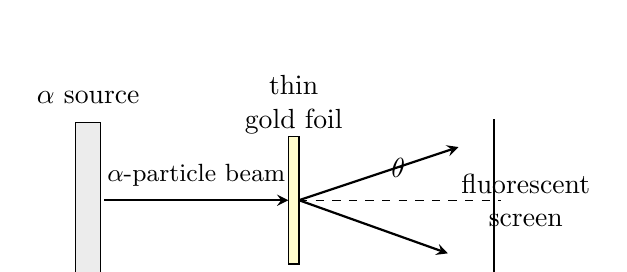
\begin{tikzpicture}[>=stealth,scale=0.9]
  \draw[fill=gray!15] (0,0) rectangle (0.35,2.2);
  \node at (0.175,2.55) {$\alpha$ source};
  \draw[->,thick] (0.4,1.1) -- (3.0,1.1);
  \node at (1.7,1.45) {\small $\alpha$-particle beam};
  \draw[fill=yellow!20] (3.0,0.2) rectangle (3.15,2.0);
  \node[align=center] at (3.075,2.45) {thin\\gold foil};
  \draw[dashed] (3.15,1.1) -- (6.0,1.1);
  \draw[->,thick] (3.15,1.1) -- (5.4,1.85);
  \draw[->,thick] (3.15,1.1) -- (5.25,0.35);
  \draw[thick] (5.9,-0.05) -- (5.9,2.25);
  \node[align=center] at (6.35,1.1) {fluorescent\\screen};
  \node at (4.55,1.55) {$\theta$};
\end{tikzpicture}
\end{center}

Most $\alpha$ particles passed through the foil essentially undeflected. Some were
deflected through appreciable angles, and a very small number were scattered through
very large angles, including particles that were effectively ``backscattered.''

The $\alpha$ particle is positively charged, so the large-angle deflections indicate
strong electrostatic repulsion from a concentrated positive charge. The conclusions
were therefore:

\begin{itemize}
    \item atoms are mostly empty space;
    \item the positive charge is concentrated in a very small region;
    \item almost all of the atomic mass is concentrated in this region;
    \item this region is the atomic nucleus, with a characteristic scale of about
    $10^{-15}\,\mathrm{m}$ compared with an atomic scale of about $10^{-10}\,\mathrm{m}$.
\end{itemize}

The experiment therefore provided decisive evidence for the nuclear model of the atom.

% =========================================================
\section{Question 3 --- Thermal radiation}

The Stefan--Boltzmann law is
\[
\Phi=\sigma T^4,
\]
where
\[
\sigma=5.67\times10^{-8}\,
\mathrm{W\,m^{-2}\,K^{-4}}.
\]

For a radiating area $A$,
\[
P=A\sigma T^4.
\]

Wien's displacement law is
\[
\lambda_{\max}T=2.90\times10^{-3}\,\mathrm{m\,K}.
\]

\subsection{(i) Temperature of a tungsten filament}

The filament is modelled as a thin strip with
\[
L=0.20\,\mathrm m,\qquad
w=0.14\,\mathrm{mm}=1.4\times10^{-4}\,\mathrm m.
\]

Using the strip area specified by the model,
\[
A=Lw
=(0.20)(1.4\times10^{-4})
=2.8\times10^{-5}\,\mathrm{m^2}.
\]

We make the simplified model assumption that the effective radiating area is the given
strip area $A=Lw$ and that the full \SI{100}{W} electrical input is emitted as thermal
radiation. Thus
\[
P=A\sigma T^4,
\]
so
\[
T=
\left(\frac{P}{A\sigma}\right)^{1/4}.
\]

Therefore
\[
T=
\left[
\frac{100}
{(2.8\times10^{-5})(5.67\times10^{-8})}
\right]^{1/4}
\approx2820\,\mathrm K.
\]

Converting to Celsius,
\[
T\approx2820-273
\approx2540^\circ\mathrm C.
\]

Thus
\[
\boxed{T\approx2540^\circ\mathrm C}.
\]

The assumptions are that the effective radiating area is $Lw$, that the full
\SI{100}{W} electrical input is radiated thermally, and that the filament behaves as
a black body. These are approximations: a real bulb also loses energy through
conduction and convection, and tungsten is not a perfect black body. The resulting
temperature is therefore an estimate, but is reasonable for the simplified model.

\subsection{(ii) Luminosity of the Sun}

The solar radius is
\[
R_\odot=695500\,\mathrm{km}=6.955\times10^8\,\mathrm m,
\]
and its surface temperature is
\[
T_\odot=5778\,\mathrm K.
\]

The surface area is
\[
A_\odot=4\pi R_\odot^2.
\]

Therefore
\[
L_\odot
=
4\pi R_\odot^2\sigma T_\odot^4.
\]

Substitution gives
\[
L_\odot
=
4\pi(6.955\times10^8)^2
(5.67\times10^{-8})(5778)^4,
\]
hence
\[
\boxed{L_\odot\approx3.84\times10^{26}\,\mathrm W}.
\]

\subsection{(iii) Solar panel on Mars}

At distance
\[
r=227.9\,\text{million km}
=2.279\times10^{11}\,\mathrm m,
\]
the Sun's radiation is spread over a sphere of area
\[
4\pi r^2.
\]

A square panel of area $a^2$ therefore receives
\[
P_{\rm received}
=
\frac{L_\odot}{4\pi r^2}a^2.
\]

If the panel efficiency is $\beta=0.20$, its useful output is
\[
P
=
\beta\frac{L_\odot}{4\pi r^2}a^2.
\]

Solving for the side length,
\[
a=
\sqrt{
\frac{4\pi P r^2}{\beta L_\odot}
}.
\]

For $P=100\,\mathrm W$,
\[
a
=
\sqrt{
\frac{4\pi(100)(2.279\times10^{11})^2}
{(0.20)(3.84\times10^{26})}
}
\approx0.92\,\mathrm m.
\]

Thus
\[
\boxed{a\approx0.92\,\mathrm m}.
\]

\subsection{(iv) Radiation from human skin}

Taking the skin temperature as
\[
T=34^\circ\mathrm C=307\,\mathrm K,
\]
Wien's law gives
\[
\lambda_{\max}
=
\frac{2.90\times10^{-3}}{307}.
\]

Hence
\[
\lambda_{\max}\approx9.45\times10^{-6}\,\mathrm m
=\boxed{9450\,\mathrm{nm}}.
\]

This lies in the
\[
\boxed{\text{infrared}}
\]
region of the electromagnetic spectrum, explaining the use of infrared cameras
for detecting heat signatures.

\subsection{(v) Spectra of hot and cool stars}

The Planck spectrum has the form
\[
B(\lambda,T)
=
\frac{2hc^2}{\lambda^5}
\frac{1}{e^{hc/(\lambda k_BT)}-1}.
\]

A qualitative sketch is shown below. The hotter blue star peaks at a shorter
wavelength and has a larger total emitted power, while the cooler red star peaks at a
longer wavelength. The total area under each curve increases with temperature because
of the $T^4$ dependence of the Stefan--Boltzmann law.

\begin{center}
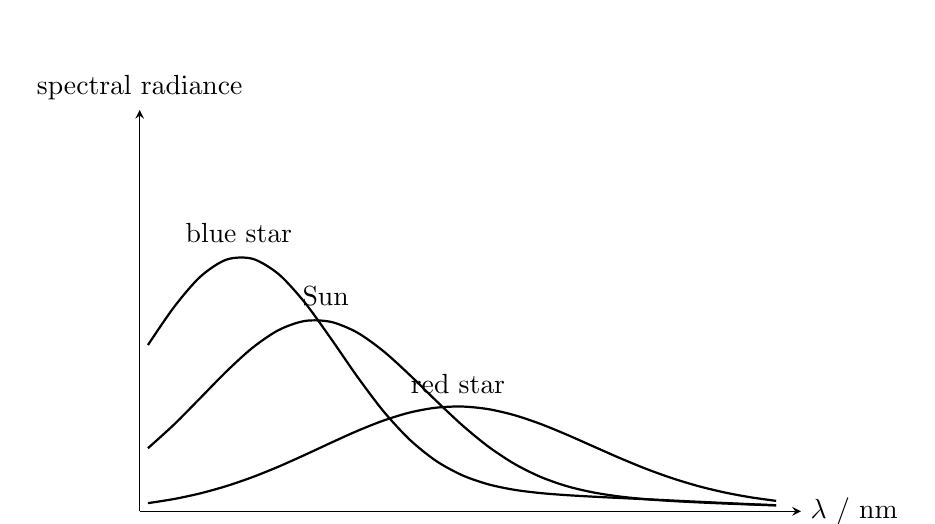
\begin{tikzpicture}[x=0.0105cm,y=0.006cm,>=stealth]
  \draw[->] (350,0) -- (1150,0) node[right] {$\lambda$ / nm};
  \draw[->] (350,0) -- (350,850) node[above] {spectral radiance};
  \draw[domain=360:1120,smooth,thick] plot (\x,{520*exp(-((\x-470)/170)^2)+35*exp(-((\x-760)/360)^2)});
  \draw[domain=360:1120,smooth,thick] plot (\x,{390*exp(-((\x-560)/190)^2)+25*exp(-((\x-820)/360)^2)});
  \draw[domain=360:1120,smooth,thick] plot (\x,{210*exp(-((\x-730)/230)^2)+15*exp(-((\x-900)/360)^2)});
  \node at (470,590) {blue star};
  \node at (575,455) {Sun};
  \node at (735,270) {red star};
\end{tikzpicture}
\end{center}

For the Sun,
\[
\lambda_{\max}
=
\frac{2.90\times10^{-3}}{5778}
\approx5.02\times10^{-7}\,\mathrm m,
\]
so
\[
\boxed{\lambda_{\max}\approx502\,\mathrm{nm}}.
\]

\subsection{(vi) Expansion into a red giant}

Initially,
\[
\lambda_{\max,\odot}\approx502\,\mathrm{nm}.
\]

For the red giant,
\[
\lambda_{\max,\mathrm{RG}}=680\,\mathrm{nm}.
\]

Using Wien's law,
\[
T_{\rm RG}
=
\frac{2.90\times10^{-3}}
{680\times10^{-9}}
\approx4265\,\mathrm K.
\]

Assuming the luminosity remains constant,
\[
L=4\pi R^2\sigma T^4=\text{constant}.
\]

Therefore
\[
R_{\rm RG}^2T_{\rm RG}^4
=
R_\odot^2T_\odot^4,
\]
giving
\[
\frac{R_{\rm RG}}{R_\odot}
=
\left(\frac{T_\odot}{T_{\rm RG}}\right)^2.
\]

Thus
\[
\frac{R_{\rm RG}}{R_\odot}
=
\left(\frac{5778}{4265}\right)^2
\approx1.84.
\]

Hence
\[
\boxed{\frac{R_{\rm RG}}{R_\odot}\approx1.84}.
\]

% =========================================================
\section{Question 4 --- Photoelectric effect}

For silver,
\[
\phi=4.3\,\mathrm{eV}.
\]

The photoelectric equation is
\[
K_{\max}=hf-\phi
=
\frac{hc}{\lambda}-\phi.
\]

\subsection{(i) Maximum wavelength}

At threshold,
\[
K_{\max}=0,
\]
so
\[
\frac{hc}{\lambda_{\max}}=\phi.
\]

Hence
\[
\lambda_{\max}
=
\frac{hc}{\phi}.
\]

Using $\phi=4.3\times1.60\times10^{-19}\,\mathrm J$,
\[
\lambda_{\max}
=
\frac{(6.63\times10^{-34})(2.998\times10^8)}
{(4.3)(1.60\times10^{-19})}
\approx2.89\times10^{-7}\,\mathrm m.
\]

Therefore
\[
\boxed{\lambda_{\max}\approx289\,\mathrm{nm}}.
\]

\subsection{(ii) Photoelectron energy for \SI{200}{nm} light}

The photon energy is
\[
E_\gamma=\frac{hc}{\lambda}.
\]

Thus
\[
K_{\max}
=
\frac{hc}{\lambda}-\phi.
\]

For $\lambda=200\,\mathrm{nm}$,
\[
K_{\max}
\approx1.91\,\mathrm{eV}.
\]

Converting to joules,
\[
K_{\max}
=
(1.91)(1.60\times10^{-19})
\approx3.06\times10^{-19}\,\mathrm J.
\]

Hence
\[
\boxed{K_{\max}\approx3.06\times10^{-19}\,\mathrm J}.
\]

\subsection{(iii) Photon absorption rate}

The incident power is
\[
P=1.00\times10^{-6}\,\mathrm W.
\]

Each photon has energy
\[
E_\gamma=\frac{hc}{\lambda}.
\]

Therefore the number absorbed per second is
\[
\dot N
=
\frac{P}{E_\gamma}
=
\frac{P\lambda}{hc}.
\]

Thus
\[
\dot N
\approx
1.01\times10^{12}\,\mathrm{s^{-1}}.
\]

So
\[
\boxed{\dot N\approx1.01\times10^{12}\,\mathrm{photons\,s^{-1}}}.
\]

\subsection{(iv) Photocurrent}

If one electron is emitted per photon,
\[
I=e\dot N.
\]

Hence
\[
I
=
(1.60\times10^{-19})
(1.01\times10^{12})
\approx1.61\times10^{-7}\,\mathrm A.
\]

Therefore
\[
\boxed{I\approx1.61\times10^{-7}\,\mathrm A}
\]
or approximately
\[
\boxed{0.16\,\mu\mathrm A}.
\]

\subsection{(v) Stopping voltage}

The stopping voltage satisfies
\[
eV_s=K_{\max}.
\]

Since $K_{\max}=1.91\,\mathrm{eV}$,
\[
\boxed{V_s\approx1.91\,\mathrm V}.
\]

% =========================================================
\section{Question 5 --- Electron diffraction}

An electron of mass $m$ and charge magnitude $e$ is accelerated through a potential
difference $V$.

\subsection{(i) Final velocity}

The electron gains kinetic energy
\[
eV.
\]

In the classical limit,
\[
eV=\frac12mv^2.
\]

Therefore
\[
v^2=\frac{2eV}{m},
\]
and
\[
\boxed{v=\sqrt{\frac{2eV}{m}}}.
\]

\subsection{(ii) Classical limit}

We require
\[
v<0.01c.
\]

Using the result above,
\[
\sqrt{\frac{2eV}{m}}<0.01c.
\]

Squaring,
\[
\frac{2eV}{m}<10^{-4}c^2,
\]
so
\[
V<
10^{-4}\frac{mc^2}{2e}.
\]

For an electron,
\[
m=9.109\times10^{-31}\,\mathrm{kg},
\qquad
e=1.60\times10^{-19}\,\mathrm C,
\]
and
\[
c=2.998\times10^8\,\mathrm{m\,s^{-1}}.
\]

Therefore
\[
\boxed{V<25.6\,\mathrm V}.
\]

Below this voltage, relativistic effects can safely be neglected.

For comparison, if one extrapolates the classical expression to very high voltages,
the discrepancy eventually becomes important. The exact relativistic kinetic energy is
\[
eV=(\gamma-1)mc^2,
\qquad
\gamma=\frac{1}{\sqrt{1-v^2/c^2}}.
\]

For example, at $V=5\,\mathrm{kV}$ the classical approximation gives
$v/c\approx0.14$, so relativistic corrections are no longer completely negligible.

\subsection{(iii) Classical de Broglie wavelength}

The de Broglie relation is
\[
\lambda=\frac{h}{p}.
\]

In the classical limit,
\[
K=\frac{p^2}{2m}.
\]

Since
\[
K=eV,
\]
we have
\[
eV=\frac{p^2}{2m}.
\]

Therefore
\[
p=\sqrt{2meV},
\]
and hence
\[
\boxed{
\lambda=\frac{h}{\sqrt{2meV}}
}.
\]

\subsection{(iv) Diffraction pattern}

The electron beam strikes a carbon disc whose atomic layers have spacing
\[
d=1.23\times10^{-10}\,\mathrm m.
\]

The screen therefore shows a diffraction/interference pattern rather than a
single classical scattering spot.

A qualitative sketch of intensity against scattering angle is

\begin{center}
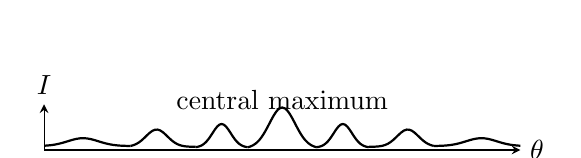
\begin{tikzpicture}[x=0.055cm,y=0.010cm,>=stealth]
  \draw[->] (-55,0) -- (55,0) node[right] {$\theta$};
  \draw[->] (-55,0) -- (-55,58) node[above] {$I$};
  \draw[smooth,thick,domain=-55:-35] plot (\x,{5+10*exp(-((\x+46)/5)^2)});
  \draw[smooth,thick,domain=-35:-20] plot (\x,{4+22*exp(-((\x+29)/3.5)^2)});
  \draw[smooth,thick,domain=-20:-8] plot (\x,{3+30*exp(-((\x+14)/3)^2)});
  \draw[smooth,thick,domain=-8:8] plot (\x,{2+52*exp(-((\x)/4.2)^2)});
  \draw[smooth,thick,domain=8:20] plot (\x,{3+30*exp(-((\x-14)/3)^2)});
  \draw[smooth,thick,domain=20:35] plot (\x,{4+22*exp(-((\x-29)/3.5)^2)});
  \draw[smooth,thick,domain=35:55] plot (\x,{5+10*exp(-((\x-46)/5)^2)});
  \node at (0,64) {central maximum};
\end{tikzpicture}
\end{center}

The maxima arise because the electron has a de Broglie wavelength
\[
\lambda=\frac hp
\]
and waves scattered from successive atomic layers interfere constructively at
particular angles.

Thus the experiment demonstrates that electrons possess wave-like properties:
they can diffract and interfere.

\subsection{(v) First diffraction peak}

For the geometry used in the problem sheet, the first-order condition is
\[
d\sin\theta=\lambda.
\]

For the first peak,
\[
\theta=10.0^\circ,
\qquad
d=1.23\times10^{-10}\,\mathrm m.
\]

Using
\[
\lambda=\frac{h}{\sqrt{2meV}},
\]
we obtain
\[
d\sin\theta
=
\frac{h}{\sqrt{2meV}}.
\]

Squaring and rearranging,
\[
V=
\frac{h^2}
{2me\,d^2\sin^2\theta}.
\]

Therefore
\[
V
=
\frac{(6.63\times10^{-34})^2}
{2(9.109\times10^{-31})(1.60\times10^{-19})
(1.23\times10^{-10})^2\sin^2(10^\circ)}
\approx3.3\times10^3\,\mathrm V.
\]

Hence
\[
\boxed{V\approx3.3\,\mathrm{kV}}.
\]

\subsection{(vi) Other diffraction peaks}

For diffraction order $n$,
\[
d\sin\theta_n=n\lambda.
\]

Thus
\[
\boxed{
\theta_n=\sin^{-1}\left(\frac{n\lambda}{d}\right)
}.
\]

For the voltage calculated above,
\[
\frac{\lambda}{d}\approx0.174.
\]

Hence
\[
\theta_n=\sin^{-1}(0.174n).
\]

The allowed positive orders are $n=1,\ldots,5$, since
\[
\frac{1}{0.174}\approx5.76.
\]

The corresponding scattering angles are approximately

\[
\boxed{
\theta
=
0^\circ,\,
\pm10.0^\circ,\,
\pm20.3^\circ,\,
\pm31.4^\circ,\,
\pm44.0^\circ,\,
\pm60.3^\circ
}.
\]

The central maximum occurs at $0^\circ$, with symmetric maxima on either side.
A qualitative sketch of the resulting pattern is

\begin{center}
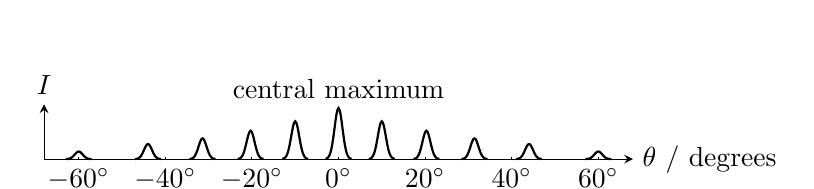
\begin{tikzpicture}[x=0.055cm,y=0.012cm,>=stealth]
  \draw[->] (-68,0) -- (68,0) node[right] {$\theta$ / degrees};
  \draw[->] (-68,0) -- (-68,58) node[above] {$I$};
  \foreach \c/\h in {-60/8,-44/16,-31.4/22,-20.3/30,-10/40,0/54,10/40,20.3/30,31.4/22,44/16,60/8}
    \draw[smooth,thick] plot[domain=\c-3: \c+3] (\x,{\h*exp(-((\x-\c)/1.3)^2)});
  \foreach \x in {-60,-40,-20,0,20,40,60}
    \draw[thin] (\x,0) -- (\x,2);
  \foreach \x/\label in {-60/$-60^\circ$,-40/$-40^\circ$,-20/$-20^\circ$,0/$0^\circ$,20/$20^\circ$,40/$40^\circ$,60/$60^\circ$}
    \node[below] at (\x,0) {\label};
  \node[above] at (0,54) {central maximum};
\end{tikzpicture}
\end{center}

Because the carbon disc and detector have finite dimensions, the real peaks have
finite widths rather than being infinitely sharp.

% =========================================================
\section{Question 6 --- Hydrogen spectral lines}

The Bohr model gives the hydrogen energy levels as
\[
\boxed{
E_n=-\frac{13.6\,\mathrm{eV}}{n^2}
}.
\]

For a transition from $n$ to $m<n$, the emitted photon has energy
\[
E_\gamma
=
E_n-E_m
\]
in magnitude, and
\[
E_\gamma=\frac{hc}{\lambda}.
\]

Equivalently, the wavelength is given by the supplied hydrogenic relation
\[
\lambda_{nm}
\approx
91.13\,\mathrm{nm}
\left(
\frac{1}{m^2}-\frac{1}{n^2}
\right)^{-1}.
\]

\subsection{(i) Lyman series: $n=3\rightarrow1$}

For $m=1$ and $n=3$,
\[
\lambda
=
\frac{91.13\,\mathrm{nm}}
{1-\frac{1}{3^2}}.
\]

Therefore
\[
\lambda\approx103\,\mathrm{nm}.
\]

Thus
\[
\boxed{\lambda\approx103\,\mathrm{nm}},
\]
which lies in the
\[
\boxed{\text{ultraviolet}}
\]
region.

\subsection{(ii) Balmer series: $n=4\rightarrow2$}

Now
\[
\lambda
=
\frac{91.13\,\mathrm{nm}}
{\frac{1}{2^2}-\frac{1}{4^2}}.
\]

Hence
\[
\lambda\approx487\,\mathrm{nm}.
\]

Therefore
\[
\boxed{\lambda\approx487\,\mathrm{nm}},
\]
which lies in the
\[
\boxed{\text{visible}}
\]
region.

\subsection{(iii) Pfund series: $n=7\rightarrow5$}

For $m=5$ and $n=7$,
\[
\lambda
=
\frac{91.13\,\mathrm{nm}}
{\frac{1}{5^2}-\frac{1}{7^2}}.
\]

Therefore
\[
\lambda\approx4660\,\mathrm{nm}.
\]

Hence
\[
\boxed{\lambda\approx4660\,\mathrm{nm}},
\]
which lies in the
\[
\boxed{\text{infrared}}
\]
region.

% =========================================================
\section*{Numerical results}

\begin{center}
\begin{tabular}{ll}
\toprule
\textbf{Part} & \textbf{Result}\\
\midrule
1(i) & $r_{\rm atom}/r_{\rm nucleus}\sim10^5$\\
1(ii) & $N_{\rm atom}\sim4.7\times10^{25}$; $N_{\rm marble}\sim4.5\times10^{25}$\\
3(i) & $T\approx2540^\circ\mathrm C$\\
3(ii) & $L_\odot\approx3.84\times10^{26}\,\mathrm W$\\
3(iii) & $a\approx0.92\,\mathrm m$\\
3(iv) & $\lambda_{\max}\approx9450\,\mathrm{nm}$ (IR)\\
3(v) & $\lambda_{\max,\odot}\approx502\,\mathrm{nm}$\\
3(vi) & $R_{\rm RG}/R_\odot\approx1.84$\\
4(i) & $\lambda_{\max}\approx289\,\mathrm{nm}$\\
4(ii) & $K_{\max}\approx3.06\times10^{-19}\,\mathrm J$\\
4(iii) & $\dot N\approx1.01\times10^{12}\,\mathrm{s^{-1}}$\\
4(iv) & $I\approx1.61\times10^{-7}\,\mathrm A$\\
4(v) & $V_s\approx1.91\,\mathrm V$\\
5(i) & $v=\sqrt{2eV/m}$\\
5(ii) & $V<25.6\,\mathrm V$\\
5(iii) & $\lambda=h/\sqrt{2meV}$\\
5(iv) & diffraction/interference pattern; electrons exhibit wave-like behaviour\\
5(v) & $V\approx3.3\,\mathrm{kV}$\\
5(vi) & $\theta=0^\circ,\pm10.0^\circ,\pm20.3^\circ,\pm31.4^\circ,\pm44.0^\circ,\pm60.3^\circ$\\
6(i) & $103\,\mathrm{nm}$ (UV)\\
6(ii) & $487\,\mathrm{nm}$ (visible)\\
6(iii) & $4660\,\mathrm{nm}$ (IR)\\
\bottomrule
\end{tabular}
\end{center}

\end{document}
